\documentclass[a4paper,12pt]{article}
\usepackage{fancyhdr}
\usepackage[MeX]{polski}
\usepackage[utf8]{inputenc}
\usepackage{amsmath,amsthm,amssymb}
\usepackage{graphicx}

\usepackage[lmargin=2.7cm]{geometry}

\pagestyle{fancy}
\lhead{e-Talk  - komunikator internetowy. Dokumentacja}
\rhead{\bfseries}



\author{Adrian Chudziński, Przemysław Gospodarczyk}
\title{e-Talk -- komunikator internetowy -- Dokumentacja}

\begin{document}

\makeatletter
    \renewcommand\@seccntformat[1]{\csname the#1\endcsname.\quad}
    \renewcommand\numberline[1]{#1.\hskip0.7em}
\makeatother

\begin{titlepage}
\begin{center}

    \textsc{Licencjacki projekt programistyczny}\\[0.1cm]
    \textsc{IIUWr 2009/2010}\\[6cm]
    Adrian Chudziński, Przemysław Gospodarczyk\\[1cm]
    \textsc{\Large e-Talk -- komunikator internetowy}\\[0.25cm]
    \textsc{\large Dokumentacja}\\[8.675cm]

    {\footnotesize
    \begin{tabular}{| c | p{4cm} | p{4.25cm} | c | }
        \hline
        Wersja  &
        Zmiany  &
        Autorzy &
        Data    \\
        \hline
        1.0                                                                   &
        Pierwsza wersja                                                       &
        \par Adrian Chudziński \par Przemysław Gospodarczyk                                                  &
        2010-03-25                                                            \\
        \hline
    \end{tabular}
    }

\end{center}
\end{titlepage}

\break

\setcounter{page}{2}

\tableofcontents

\break
\section[Słownik pojęć]{Słownik pojęć}
\noindent\textbf{America Online} (AOL) -- największy amerykański dostawca usług internetowych. Jeden z pierwszych wydawców elektronicznego biuletynu informacyjnego (BBS) w USA, który od 1995 roku jest dostępny również w Internecie. W 1998 roku wykupił firmę Netscape -- producenta przeglądarki Netscape Navigator.\\

\noindent\textbf{API} (\textit{Application Programming Interface}) -- zbiór konwencji wywoływania funkcji określających sposób dostępu do danej usługi przez system operacyjny oraz lista dostępnych funkcji wraz z opisem znaczenia ich parametrów.\\

\noindent\textbf{Commodore 64} -- model popularnego w latach osiemdziesiątych domowego komputera 8-bitowego firmy Commodore. Oparty na procesorach 6510 lub 8502 (w zależności od wersji), wyposażony w 64 KB pamięci operacyjnej RAM oraz odrębne procesory przetwarzające dane wejściowe i wyjściowe, obraz oraz dźwięk, co odciążało jednostkę centralną i umożliwiało tworzenie wydajnego oprogramowania.\\

\noindent\textbf{Emotikony} (ang. \textit{emoticons}) -- zestaw symboli wyrażających emocje, używanych w wiadomościach przesyłanych pocztą elektroniczną, przez komunikator internetowy, w grupach dyskusyjnych i w wiadomościach SMS.\\

\noindent\textbf{Excite} -- wyszukiwarka internetowa autorstwa firmy o tej samej nazwie, która została w roku 1999 wykupiona przez amerykańską firmę At Home.\\

\noindent\textbf{Extensible Messaging and Presence Protocol} (dawniej Jabber) -- protokół komunikacji oraz powiadamiania o obecności w czasie rzeczywistym oparty na języku XML. Głównym zastosowaniem Extensible Messaging and Presence Protocol jest wymiana wiadomości w komunikatorach internetowych. Serwery XMPP umożliwiają także za pomocą tzw. transportów komunikację z użytkownikami innych protokołów, np. Gadu-Gadu, Tlen.pl, ICQ i MSN Messenger.
Protokół jest również stosowany w systemie blogowania Jogger przez XMPP.\\

\noindent\textbf{Google Talk} -- komunikator internetowy i usługa VoIP amerykańskiej firmy Google. Google Talk działa od 24 sierpnia 2005 roku. Wygląd programu (kolorystyka, układ tabel, czcionki) jest stylizowany na interfejs graficzny poczty elektronicznej Gmail.\\

\noindent\textbf{Interfejs graficzny} (ang. \textit{graphical interface, GUI}) -- dominująca obecnie odmiana interfejsu użytkownika, w którym kontakt z komputerem i sterowanie programami odbywa się za pomocą okien, ikon, przycisków, suwaków i rozmaitych menu. Interfejs graficzny jest obsługiwany za pomocą myszy i sprzężonego z nią kursora; możliwe jest też używanie w interfejsie graficznym operacji klawiszowych (skrótów klawiaturowych).\\

\noindent\textbf{Jabber} -- patrz Extensible Messaging and Presence Protocol.\\

\noindent\textbf{Komunikator internetowy} (ang. \textit{instant messenger}) -- program komputerowy pozwalający na przesyłanie natychmiastowych komunikatów (ang. \textit{instant messaging}) między dwoma lub więcej komputerami poprzez sieć Internet. Od poczty elektronicznej różni się tym, że oprócz samej wiadomości, przesyłane są także informacje o obecności użytkowników, co zwiększa znacznie szansę na prowadzenie bezpośredniej konwersacji.\\

\noindent\textbf{MSN} (ang. \textit{MicroSoft Network}) -- serwis internetowy firmy Microsoft, który oferuje pocztę elektroniczną oraz fora dyskusyjne dotyczące różnych dziedzin i tematów.\\

\noindent\textbf{PETSCII} (ang. \textit{PET Standard Code of Information Interchange}) -- rodzaj zbioru znaków ASCII z 1977 roku znany również jako CBM ASCII, używany w 8-bitowych komputerach Commodore 64.\\

\noindent\textbf{Pidgin} (dawniej GAIM) -- wielosystemowy komunikator internetowy obsługujący wiele protokołów transmisyjnych. Pidgin jest oprogramowaniem bezpłatnym (o otwartym kodzie), dostępnym na warunkach GNU GPL i został zbudowany przez Marka Spencera dla systemów uniksowych, jednak obecnie jest dostępny także dla systemów Windows, MacOS, SkyOS oraz Qt Extended (dla urządzeń PDA).\\

\noindent\textbf{Serwis społecznościowy (portal społecznościowy)} -- rodzaj interaktywnych stron WWW, które są współtworzone przez sieci społeczne osób podzielających wspólne zainteresowania lub chcących poznać zainteresowania innych. Większość portali społecznościowych dostarcza użytkownikom wielu sposobów komunikacji, np. czaty, komunikatory, listy dyskusyjne, blogi i fora dyskusyjne.\\

\noindent\textbf{Sieć P2P} (ang. \textit{peer--to--peer}) -- sieć partnerska, architektura sieciowa oparta na równoważności wszystkich jej węzłów. W sieci P2P każdy komputer dysponuje podobnymi możliwościami oraz może inicjować połączenia. Nie ma ustalonej hierarchii ani centralnego serwera. Ten sam komputer może równocześnie pełnić rolę serwera i klienta, czyli pobierać dane z innych komputerów i udostępniać swoje zasoby wszystkim pozostałym komputerom.\\

\noindent\textbf{Tablica dzielona} (ang. \textit{shared whiteboard}) -- miejsce na dysku dostępne dla wielu użytkowników jednocześnie. Wersje poszczególnych użytkowników są synchronizowane w czasie zbliżonym do rzeczywistego.\\

\noindent\textbf{Twitter} -- darmowy serwis społecznościowy udostępniający usługę mikroblogowania umożliwiającą użytkownikom wysyłanie oraz odczytywanie tak zwanych tweetów.\\ Tweet to krótka, nie przekraczająca 140 znaków wiadomość tekstowa wyświetlana na stronie użytkownika oraz dostarczana pozostałym użytkownikom, którzy obserwują dany profil. Użytkownicy mogą dodawać krótkie wiadomości do swojego profilu z poziomu strony głównej serwisu, wysyłając wiadomości SMS lub korzystając z zewnętrznych aplikacji.\\

\noindent\textbf{Ubique} -- firma produkująca oprogramowanie do błyskawicznej komunikacji. Najbardziej znaną aplikacją Ubique jest Virtual Places Chat, a użyta technika znalazła zastosowanie w aplikacji Lotus Sametime firmy IBM. Obecnie Ubique jest częścią IBM Haifa Labs.\\

\noindent\textbf{Yahoo} -- jeden z najpopularniejszych portali internetowych należący do amerykańskiej firmy Yahoo. Oprócz hierarchicznego katalogu kategorii tematycznych zawiera także mechanizm przeszukiwania zasobów Internetu.\\

\noindent\textbf{Yahoo Messenger} -- komunikator internetowy firmy Yahoo. Pierwsza wersja komunikatora ukazała się 9 marca 1998 roku pod nazwą Yahoo Pager.\\

\section[Wstęp, Komunikatory jako zjawisko społeczne]{Wstęp, Komunikatory jako zjawisko społeczne}
Podstawowymi cechami Internetu są globalność i masowość.
Istotną cechą Internetu jest masowość jego użytkowników, którzy traktują go nierzadko jako jedyne okno na świat.
Użytkownicy, korzystając z Internetu w poszukiwaniu informacji, danych lub szukając kontaktu z innymi ludźmi w świecie wirtualnym nie tylko rozwijają globalną Sieć, ale stają się również jej integralną i nieodzowną częścią.
Człowiek jako istota społeczna uzewnętrznia swoją potrzebę komunikacji poprzez pośrednią i bezpośrednią wymianę informacji z innymi ludźmi. Komunikacja sieciowa jest pośrednia i pozbawiona komunikatów niewerbalnych takich jak:
ton głosu, mimika, wygląd i zachowanie. Wyżej wymienione aspekty komunikacji sieciowej jednoznacznie wskazują na jej ograniczoność w stosunku do bezpośrednich kontaktów międzyludzkich. Niewerbalna komunikacja może wzmacniać, osłabiać, a nawet negować przekazy werbalne. W związku z tym komunikaty werbalne mają ogromne znaczenie w komunikacji i mogą stać się ważniejsze niż treść wypowiedzi. Internet powoduje, że wzajemne kontakty stają się bardziej powierzchowne i tracą ważną część swojego charakteru.

\par Komunikacja sieciowa ma jednak swoje zalety, które przez wiele osób są marginalizowane.
Najważniejszą cechą komunikacji internetowej jest jej anonimowość. Użytkownicy często fałszują swoje dane osobowe lub nie podają ich w ogóle. Możliwa jest błyskawiczna zmiana tożsamości. Bezpośrednia komunikacja w świecie rzeczywistym jest znacznie trudniejsza niż internetowa. Ludzie hamowani przez nieśmiałość oraz lęk przed odrzuceniem w dużej mierze rezygnują z tego typu komunikacji. Anonimowość -- często złudna -- powoduje, że wyżej wymienione czynniki tracą na znaczeniu. Badania japońskich naukowców z Ochanomizu University \cite {OU} dotyczące studentów dowodzą, że relacje interpersonalne w życiu wymagają pewnych umiejętności społecznych oraz orientacji na innych.

\par Komunikatory internetowe stały się bardzo popularną formą komunikacji wśród młodzieży, grupy społecznej, która najbardziej potrzebuje kontaktów z rówieśnikami oraz akceptacji i dowartościowania. Współczesna młodzież jest bardziej spragniona relacji interpersonalnych niż pokolenie urodzone w latach sześćdziesiątych i siedemdziesiątych.
Według Stevena Gerali, szefa chicagowskiego \emph{Department of Youth Ministry \& Adolescent Studies} \cite {OU} współcześni młodzi ludzie chcą intymności, stałości oraz bezpiecznych związków z innymi. Przede wszystkim pragną być doceniani i chronieni. Ważnym czynnikiem staje się anonimowość, która zapewnia młodemu użytkownikowi bezpieczeństwo oraz do pewnego stopnia bezkarność i łatwość w poznawaniu oraz komunikacji z ludźmi z całego świata.
W Internecie zawiera się przyjaźnie, przeżywa miłość, zdobywa informacje i nowe hobby.\\
Nie każdy nastolatek jest wyposażony w wymagany przez komunikację bezpośrednią zestaw cech. Komunikatory internetowe ich nie wymagają. Każdy użytkownik może przedstawić siebie w zupełnie inny, wymarzony przez siebie sposób, koloryzując rzeczywistość. Nastolatkowie utrzymujący takie kontakty zwiększają swoją pewność siebie, która będzie procentować w życiu dorosłym.

\par Wbrew powszechnym opiniom, z komunikatorów internetowych i portali społecznościowych korzystają jednak coraz częściej ludzie dorośli, których przyciąga darmowość usługi oraz prostota obsługi. W artykule \emph{Rosja też ćwierka}, zamieszczonym w tygodniku \emph{Polityka} \cite{PO}, autorzy Marek Ostrowski i Adam Szostkiewicz opisują portal społecznościowy \textbf{Twitter} jako miejsce wymiany zdań głównie między ludźmi pełnoletnimi.\\
Za niespodziankę można uznać wielką popularność Twittera zważywszy, że umożliwia on wysyłanie wiadomości o długości do 140 znaków, co powinno stanowić poważne utrudnienie w korespondowaniu. Użytkownicy Twittera nie wykorzystują go jednak do poważnych rozmów, lecz do bezzwłocznego pisania o tym, co ich w danym momencie interesuje i emocjonuje. Ponadto Twitter pozwala na sprawdzenie, co interesuje innych oraz, według psychologa z Uniwersytetu Warszawskiego Jana Zająca, sprzyja rozmowom o niczym w celu podtrzymania relacji towarzyskich z innymi ludźmi.\\
Według pobieżnej analizy przeprowadzonej przez autorów wspomnianego artykułu, prasa jest ciągle bardziej opiniotwórcza i dostarcza więcej informacji.\\
Twitter sprzyja również rozwojowi literatury mądrości (ang. \textit{wisdom literature}), czyli pisaniu aforyzmów, czego nie można już uznać za prymitywną formę komunikacji. Wysyłanie krótkich wiadomości nie tylko zaśmieca głowę, ale również potrafi zmobilizować do myślenia.

\par Komunikatory internetowe pomagają w życiu społecznym osobom niepełnosprawnym, ludziom, którzy z powodu swojego kalectwa posiadają niskie zdanie o sobie oraz obawiają się odrzucenia z powodu swojej odmienności. W Internecie chory człowiek nie obawia się zdemaskowania prawdy o sobie ani o swojej ewentualnej nieatrakcyjności fizycznej spowodowanej kalectwem.

\par Istnieje wiele teorii na temat wypierania kontaktów w świecie rzeczywistym przez kontakty w Internecie, a wpływ komunikatorów internetowych na życie społeczne człowieka jest oceniany przez naukowców bardzo niejednoznacznie.\\
Socjolog Sherry Turkle w swojej książce \emph{Life on the Screen} \cite{ST} udowodniła, że rozwój komunikatorów internetowych i portali społecznościowych prowadzi najpierw do wyobcowania poszczególnych jednostek, a w konsekwencji do społecznego autyzmu i nadmiernego indywidualizmu internautów.
Według autorki internauci stają się leniwi, nie podejmują trudów związanych z utrzymywaniem kontaktów społecznych w świecie rzeczywistym.\\
Z drugiej strony, według kanadyjskiego socjologa Barry'ego Wellmana uznawanego powszechnie za jednego z najwybitniejszych badaczy współczesnej cywilizacji, w tym także Internetu, komunikacja sieciowa uzupełnia kontakty, nie eliminując jednocześnie podstawowych form komunikacji, np. spotkań bezpośrednich \cite{OU}. Według jego badań internaci częściej interesują się polityką i biorą udział w życiu społecznym.

\par Fakt, że pomimo dużej liczby komunikatorów internetowych na rynku, autorzy projektu tworzą kolejne narzędzie do internetowego plotkowania należy usprawiedliwić ogromnym zainteresowaniem tego typu aplikacjami oraz, co za tym idzie, ogromnymi pieniędzmi za reklamy. Przed napisaniem własnego oprogramowania autorzy przeprowadzili analizę komunikatorów internetowych dostępnych na polskim rynku, aby nie powielać błędów konkurencji i wykorzystać najlepsze pomysły.

\section[Historia komunikatorów]{Historia komunikatorów}
Pomysł na komunikator błyskawicznie przesyłający i odbierający wiadomości jest starszy niż sama idea Internetu. Jest związany z wielodostępnymi systemami operacyjnymi z połowy lat sześćdziesiątych. Systemy operacyjne CTSS i Multics były używane do szybkiej i prostej komunikacji pomiędzy użytkownikami pracującymi na tej samej maszynie jednocześnie.

\par Wraz z pojawieniem się, a następnie rozwojem Internetu protokół wymiany wiadomości został poszerzony o możliwość komunikacyjne globalnej sieci. W pierwszych komunikatorach, wydanych w 1983 roku używano protokołu
partnerskiego (\textbf{P2P}). Przykładami takich programów były: talk, ytalk oraz ntalk.
W niektórych komunikatorach zastosowano architekturę klient-serwer. Przykładami aplikacji typu klient-serwer były: talker (1984) oraz IRC (1988).

\newpage
Na fali popularności \textbf{Bulletin Board System} w latach osiemdziesiątych pojawiło się wiele serwisów komputerowych udostępniających na maszynach miejsca, w których można umieszczać i czytać ogłoszenia, obsługiwać własną skrzynkę pocztową oraz pobierać i przesyłać pliki.
Przykładem takiego serwisu jest Freelancin' Roundtable działający przez ponad 3 lata od października 1984 roku do listopada 1987 roku.

\par W drugiej połowie lat osiemdziesiątych i na początku lat dziewięćdziesiątych internetowy serwis Quantum Link oferował użytkownikom \textbf{Commodore 64} przesyłanie wiadomości między połączonymi użytkownikami. Wiadomości nazywane On-Line Messages (w skrócie OLM) pojawiały się na żółtym pasku wraz z informacją o nazwie nadawcy. Quantum Link wykorzystywał znaną z Commodore 64 grafikę tekstową \textbf{PETSCII} (zob. słownik). Interfejs graficzny Quantum Link  (o ile w ogóle mogła być o nim mowa w tym przypadku) był nieporównanie gorszy z możliwościami późniejszych tego typu programów, które działały pod systemami Windows i Unix.\\
Późniejsza wersja Quantum Link znana jako \textbf{America Online} posiadała serwis \textbf{AOL Instant Messenger} (w skrócie AIM) do przesyłania wiadomości i zyskała większą popularność niż poprzedniczka.

\par Pierwsze nowoczesne komunikatory internetowe z interfejsem graficznym, które wyglądem i możliwościami przypominały znane z dzisiejszych czasów zaczęły powstawać od połowy lat dziewięćdziesiątych.\\
Przykładem takiej aplikacji jest PowWow (1998), który był jednym z pierwszych komunikatorów internetowych działających pod systemem Windows. Program zawierał wiele nietypowych i innowacyjnych dodatków takich jak:
\begin{itemize}
    \item[--] odtwarzacz plików dźwiękowych w formacie WAV;
    \item[--] wbudowany syntezator mowy;
    \item[--] program przysyłania mowy w protokole VoIP;
    \item[--] program do komunikacji według protokołów POP i SMTP;
    \item[--] program obsługujący \textbf{tablicę dzieloną} (zob. słownik), miejsce na dysku dostępne dla wielu użytkowników jednocześnie.
\end{itemize}
Innym przykładem jest działający również pod Windows \textbf{ICQ} (1996), wyprodukowany przez izraelską firmę Mirabilis. ICQ działa do dzisiaj, a w 1998 roku prawa do ICQ wykupił AOL za 407 milionów dolarów. W serwisie ICQ jest obecnie ponad 100 milionów zarejestrowanych kont, a AOL przyznano prawa do dwóch patentów dotyczących przesyłania informacji przez Internet. Angielski zwrot Instant Messenger, a także skrót IM, w Stanach Zjednoczonych jest własnością AOL i nie może być używany przez inne firmy. Działający pod wszystkimi najpopularniejszymi systemami operacyjnymi komunikator GAIM został z tego powodu przemianowany w 2007 roku na \textbf{Pidgin}.

W tym czasie inne firmy, wśród nich \textbf{Excite}, \textbf{MSN}, \textbf{Ubique} i \textbf{Yahoo}, pracowały nad swoim własnym oprogramowaniem.
Wszystkie aplikacje wyprodukowane przez te firmy miały własne, niezależne protokoły przesyłania wiadomości, co powodowało, że użytkownicy musieli korzystać ze wielu komunikatorów, aby móc połączyć się z każdą siecią.

\par W 1998 roku IBM wprowadził na rynek IBM Lotus Sametime oparte na technologii zastosowanej w komunikatorze firmy Ubique. Oprócz podstawowych, typowych funkcji oprogramowanie IBM oferowało następujące nowości:
\begin{itemize}
    \item[--] archiwizowanie rozmów;
    \item[--] możliwość organizowania internetowych wideokonferencji;
    \item[--] chat;
    \item[--] możliwość wykorzystania kodeków graficznych i dźwiękowych;
    \item[--] możliwość łączenia się z innymi sieciami, takimi jak: AOL Instant Messenger, \textbf{Yahoo Messenger}, \textbf{Google Talk} oraz serwisami opartymi na XMPP;
    \item[--] otwarty interfejs programowy (API), umożliwiający integrację z innymi tego typu aplikacjami.
\end{itemize}

W 2000 roku na rynek wprowadzono program \textbf{Jabber} z powszechnie dostępnym kodem źródłowym oraz standardowy protokół \textbf{Extensible Messaging and Presence Protocol} (w skrócie XMPP). Serwery XMPP potrafiły działać jak bramy (ang. gateway) do innych protokołów wymiany wiadomości, w związku z czym wystarczyła jedna aplikacja typu klient, aby korzystać z wielu sieci. Serwery XMPP obsługiwały wszystkie najpopularniejsze wówczas protokoły.


\section[Przegląd najpopularniejszych komunikatorów na polskim rynku]{Przegląd najpopularniejszych komunikatorów na polskim rynku}
Autorzy projektu wykonali przegląd rynku komunikatorów internetowych w Polsce, aby wybrać najlepsze funkcjonalności dla swojej aplikacji i uniknąć powielania błędów konkurencji.
Według ankiety przeprowadzonej przez serwis \textbf{idg.pl} \cite{ID} najpopularniejszym komunikatorem w Polsce jest Gadu-Gadu, którego używa aż 76\% internautów. Drugie miejsce zajął Tlen (niecałe 14\%). Pozostałe komunikatory, w tym znane na całym świecie ICQ, cieszą się popularnością jednoprocentową.
Poniżej przeanalizowano najpopularniejsze komunikatory internetowe w naszym kraju.

\subsection[Gadu-Gadu]{Gadu-Gadu}
Gadu-Gadu jest najpopularniejszym komunikatorem internetowym w Polsce. Pierwsza wersja programu pojawiła się 15 sierpnia 2000 roku i jest to pierwszy polski komunikator internetowy. Premiera spotkała się ze stosunkowo dużym zainteresowaniem -- już pierwszego dnia konta założyło ponad 10 tysięcy użytkowników. Od dnia premiery użytkowników przybywa w szybkim tempie. Po roku od premiery Gadu-Gadu miało ćwierć miliona użytkowników.
Obecnie Gadu-Gadu posiada ponad 6 milionów zarejestrowanych kont. Każdego dnia, użytkownicy Gadu-Gadu wymieniają między sobą ok. 300 milionów wiadomości.\\
Na przykładzie programu Gadu-Gadu można z łatwością zauważyć, że najważniejszą cechą komunikatora internetowego jest jego masowość. Duża liczba zarejestrowanych użytkowników przyciąga innych użytkowników, którzy chcą mieć kontakt z jak największą liczbą ludzi (tzw. efekt kuli śnieżnej). Polski rynek komunikatorów internetowych rozwija się wraz z rozwojem Internetu w Polsce.\\
Drugą istotną cechą, która stawia Gadu-Gadu na 1. miejscu wśród komunikatorów internetowych w Polsce jest łatwość instalacji, konfiguracji i użytkowania. Jeżeli program ma być masowy, to używać go będą również mniej zaawansowani użytkownicy, dla których ta cecha może okazać się najistotniejsza przy wyborze komunikatora.\\
Ciekawym pomysłem twórców było uruchomienie serwisu społecznościowego \textbf{MojaGeneracja.pl}, który stał się serwisem integracyjnym dla użytkowników chcących poznać i wymieniać wiadomości z nieznanymi im dotąd osobami. Ponadto istnieje publiczny katalog użytkowników Gadu-Gadu oraz wyszukiwarka wykorzystująca dane osobowe podawane podczas rejestracji konta. Twórcy Gadu-Gadu na oficjalnej stronie chwalą się rolą, jaką odgrywa ich komunikator w życiu wielu ludzi:
,,Coraz więcej osób poznaje się dzięki Gadu-Gadu. Zawierane są pierwsze małżeństwa, ale też i pierwsze rozwody.''\cite{GG}\\
Gadu-Gadu posiada jednak pewne wady, które ze względu na wyżej wymienione zalety są marginalizowane przez mniej wymagających użytkowników lub niedostrzegane przez mniej zaawansowanych użytkowników.\\
Oryginalna wersja programu, bezpośrednio po instalacji zawiera tylko niezbędne funkcjonalności, które w dzisiejszych czasach można uznać za podstawowe. Istnieje jednak możliwość zainstalowania różnego rodzaju nieoficjalnych dodatków, które mogą rozszerzyć możliwości standardowego Gadu-Gadu.\\
Gadu-Gadu jest aplikacją darmową. Niestety wraz ze wzrostem popularności rośnie również liczba reklam, które program w najnowszej wersji wyświetla praktycznie przy każdej możliwej okazji. Warto również dodać, że z powodu dużej liczby wysyłanych wiadomości, serwer aplikacji nie daje sobie rady z przetwarzaniem dużej liczby zapytań, co powoduje chwilowe przerwy w dostępie do komunikatora.\\
Pomimo ograniczonej funkcjonalności, irytujących reklam i przejściowych problemów technicznych, Gadu-Gadu niepodzielnie rządzi na polskim rynku komunikatorów internetowych, dystansując również zagraniczną konkurencję.

\subsection[Tlen]{Tlen}
Tlen jest polskim komunikatorem internetowym serwisu o2.pl. Pierwsza wersja programu pojawiła się w październiku 2001 roku. Obecnie, jak podaje serwis \cite{TL} na Tlenie zarejestrowanych jest ponad 1.5 miliona użytkowników.\\
Program realizuje właściwie wszystkie funkcjonalności znane z Gadu-Gadu oraz zawiera istotne rozszerzenia, których brakuje zwycięzcy rankingu, np.
\begin{itemize}
    \item[--] połączenia wideo,
    \item[--] połączenia telefoniczne,
    \item[--] czaty,
    \item[--] konferencje.
\end{itemize}
Ciekawym dodatkiem są proste gry internetowe, w których mogą uczestniczyć użytkownicy oraz tablica dzielona, na której użytkownicy mogą wspólnie rysować. Ponadto, na rynku istnieje wiele nieoficjalnych rozszerzeń wzbogacających funkcjonalności i wygląd komunikatora.\\
Aby przekonać do siebie użytkowników Gadu-Gadu, których jest więcej, Tlen jest w pełni kompatybilny z siecią Gadu-Gadu obsługując protokół GG. Oznacza to, że można wymieniać wiadomości z użytkownikami Gadu-Gadu, którzy nie mają zainstalowanego komunikatora Tlen. Oczywiście wtedy możliwości komunikacji zostają zredukowane do tego, co oferuje oryginalna wersja Gadu-Gadu. Ponadto istnieją dodatkowe rozszerzenia pozwalające nawiązać tekstową łączność z użytkownikami sieci ICQ i Jabber.\\
Tlen jest aplikacją darmową, której wadą są reklamy.

\subsection[AQQ]{AQQ}
Powstały w czerwcu 2007 roku AQQ realizuje najwięcej funkcjonalności ze wszystkich polskich komunikatorów internetowych. Liczne rozszerzenia (oficjalne i nieoficjalne) bogatej w funkcjonalności wersji podstawowej powodują, że program można uznać za medialno--komunikacyjną hybrydę. AQQ oprócz wszystkich podstawowych funkcji komunikatora internetowego oferuje również:
\begin{itemize}
    \item[--] odtwarzacz audio-wideo,
    \item[--] organizator,
    \item[--] program TV,
    \item[--] tablicę dzieloną,
    \item[--] monitor pobranych danych dla użytkowników Neostrady,
    \item[--] monitor wewnętrznych zasobów komputera.
\end{itemize}
Inną zaletą AQQ są częste aktualizacje i stosunkowo szybko poprawiane błędy.\\
AQQ oferuje komunikację z następującymi sieciami: Gadu-Gadu, Tlen, Jabber, ICQ oraz Skype.\\
Największą wadą, która przesądza o mniejszej popularności AQQ, oprócz reklam, jest izolacja użytkowników tej sieci.
Żaden z dostępnych komunikatorów internetowych nie obsługuje protokołu AQQ, co oznacza, że użytkownik tego komunikatora
nie może wymieniać wiadomości z poziomu swojego konta AQQ z użytkownikami innych sieci. W związku z powyższym w przypadku chęci komunikowania się z użytkownikami innych sieci, użytkownicy AQQ nie mogą całkowicie zrezygnować z kont na innych serwerach i muszą łączyć się z nimi przez AQQ.

\section[Planowane funkcje aplikacji e-Talk]{Planowane funkcje aplikacji}
Poniższy opis zawiera funkcje, które powinien realizować e-Talk. Każda funkcja składa się z nazwy, opisu i priorytetu. Priorytet określa, jak ważna jest realizacja danej funkcji. W opisie uwzględniono 3 rodzaje priorytetów: wysoki, średni i niski.
\subsection[Rozpoczynanie rozmowy]{Rozpoczynanie rozmowy}
Priorytet: wysoki.\\

Użytkownik A rozpoczyna rozmowę z użytkownikiem B. Użytkownik B powinien zostać o tym fakcie poinformowany. Użytkownik B nie musi akceptować rozmowy. Informacja zwrotna o decyzji użytkownika B powinna zostać wysłana do osoby rozpoczynającej rozmowę.

\subsection[Prowadzenie rozmowy]{Prowadzenie rozmowy}

Priorytet: wysoki.\\

Dwóch użytkowników może swobodnie prowadzić rozmowę, wymieniając komunikaty tekstowe.

\subsection[Zmiana stanu użytkownika]{Zmiana stanu użytkownika}

Priorytet: wysoki.\\

Każdemu użytkownikowi jest przypisany stan, który może dowolnie zmieniać. W aplikacji E-Talk będą dostępne stany: ,,dostępny'', ,,niedostępny'', ,,zaraz wracam'' oraz ,,niewidoczny''. Stan użytkownika pokazywany jest wszystkim innym użytkownikom. Nie dotyczy to jednak stanu ,,niewidoczny'', użytkownik w tym stanie jest widoczna dla innych użytkowników, podobnie jak użytkownik w stanie ,,niedostępny''.

\subsection[Lista kontaktów]{Lista kontaktów}

Priorytet: wysoki.\\

Użytkownicy powinni dysponować samodzielnie definiowaną listą kontaktów. Lista może być dowolnie modyfikowana przez użytkownika.

\subsection[Zakładanie konta]{Zakładanie konta}

Priorytet: wysoki.\\

Osoby nie posiadające konta na serwerze aplikacji mogą przy pierwszym uruchomieniu programu założyć nowe konto. W tym celu muszą wypełnić krótki formularz, podając podstawowe dane osobowe.

\subsection[Zmiana danych profilu]{Zmiana danych profilu}

Priorytet: wysoki.\\

Użytkownik może dowolnie zmieniać dane zawarte w swoim profilu.

\subsection[Podstawowe funkcje edytora tekstu]{Podstawowe funkcje edytora tekstu}

Priorytet: wysoki.\\

Użytkownik powinien mieć możliwość prostego formatowania tekstu swojej wiadomości.
Przewiduje się następujące funkcje:
\begin{itemize}
    \item[--] zmiana rodzaju, wielkości i stylu czcionki;
    \item[--] zmiana koloru tekstu;
    \item[--] kopiowanie, wklejanie i wycinanie tekstu.
\end{itemize}

\subsection[Wyszukiwanie użytkowników]{Wyszukiwanie użytkowników}
Priorytet: średni.\\

Użytkownik może szukać innych użytkowników, podając fragment ich danych osobowych.

\subsection[Obsługa protokołu GG]{Obsługa protokołu GG}
Priorytet: średni.\\

W związku z popularnością komunikatora Gadu-Gadu, dobrze by było, aby użytkownik e-Talk miał możliowość tekstowej łączności z użytkownikami tego najpopularniejszego komunikatora w naszym kraju.

\subsection[Import oraz eksport listy kontaktów]{Import oraz eksport listy kontaktów}

Priorytet: średni.\\

Aplikacja E-Talk umożliwia na eksportowanie listy kontaktów do pliku lub serwera oraz import z pliku lub serwera.
\subsection[Zapisywanie i przeglądanie archiwum rozmów]{Zapisywanie i przeglądanie archiwum rozmów}
Priorytet: średni.\\

Użytkownik powinien mieć możliwość przeglądania treści swoich poprzednich rozmów.

\subsection[Wklejanie obrazów do tekstu]{Wklejanie obrazów do tekstu}

Priorytet: niski.\\

Użytkownik powinien mieć możliwość dodania do swojego tekstu obrazu pobranego z dysku twardego.
Przewiduje się obsługę wszystkich najpopularniejszych formatów graficznych.
\subsection[Przesyłanie plików]{Przesyłanie plików}

Priorytet: niski.\\

Dwóch rozmawiających ze sobą użytkowników powinno mieć możliwość przesyłania między sobą plików.
\subsection[Wyświetlanie emotikonów]{Wyświetlanie emotikonów}

Priorytet: niski.\\

Aplikacja E-Talk powinna zamieniać pewne określone ciągi znaków zapisane w tekście wiadomości na emotikony, które
wyrażają w sposób symboliczny wyraz twarzy użytkownika.

\section[Dokumentacja użytkownika]{Dokumentacja użytkownika}






\section[Model konceptualny bazy danych]{Model konceptualny bazy danych}
\subsection[Profil klienta]{Profil klienta}
Do tej kategorii należą wszyscy klienci, zarejestrowani w systemie.
Użytkownicy powinni mieć dostęp jedynie do swoich kont. Nie powinni
mieć dostępu do żadnych danych innych użytkowników systemu.
Od klienta nie wymaga się żadnej wcześniejszej wiedzy o systemie. Każdy klient dostanie
podręcznik użytkownika zawierający opis wszystkich możliwości systemu.
Ważne jest, aby opis był zrozumiały nawet dla bardzo niedoświadczonych użytkowników.

\subsection[Administratorzy systemu]{Administratorzy systemu}
Administratorzy, to osoby odpowiedzialne za prawidłowe działanie systemu i zarządzanie bazą danych.
Administratorzy powinni zostać gruntownie przeszkoleni tak, aby mogli sprawnie
zarzadzać systemem.\\
Administratorzy mają dostęp do wszystkich danych związanych z działaniem systemu i nieograniczone uprawnienia związane
z modyfikowaniem zawartości bazy danych.
Informacje o klientach powinni otrzymywać jedynie w sytuacjach, w których
jest to niezbędne.

\subsection[Opis encji]{Opis encji}
\subsubsection[Użytkownik]{Użytkownik}
Relacja \texttt{użytkownik} przechowuje podstawowe informacje o klientach, które są konieczne do prawidłowego działania systemu uwierzytelniania. Relacja zawiera kolejno następujące atrybuty:
\begin{itemize}
    \item[--] numer konta, który jest kluczem publicznym relacji \texttt{użytkownik} i jest automatycznie generowany przez sekwencję \texttt{num\_gen} po rejestracji klienta;
    \item[--] unikatową nazwę użytkownika, która jednoznacznie określa klienta w bazie danych;
    \item[--] hasło, które użytkownik podaje podczas rejestracji składające się z co najmniej 6 znaków alfanumerycznych;
    \item[--] status, możliwe wartości: ,,Dostepny'', ,,Niedostepny'', ,,Zaraz wracam'' i ,,Niewidoczny''.
\end{itemize}

\subsubsection[Dane]{Dane}
Relacja \texttt{dane} przechowuje dodatkowe informacje o kliencie, które nie są konieczne do prawidłowego działania systemu. Dane mogą okazać się jednak pomocne przy wyszukiwaniu użytkowników systemu e-Talk. Relacja zawiera kolejno następujące atrybuty:
\begin{itemize}
    \item[--] numer konta, który jest kluczem publicznym relacji \texttt{użytkownik} i jest kluczem obcym z relacji \texttt{użytkownik};
    \item[--] nazwisko, które jest polem wymaganym do wypełnienia podczas rejestracji;
    \item[--] imię, które jest polem wymaganym do wypełnienia podczas rejestracji;
    \item[--] kod pocztowy, który nie jest wymaganym polem do wypełnienia podczas rejestracji. Poprawność
              tego pola jest sprawdzana na podstawie domeny \texttt{kod\_type} opartej na prostym wyrażeniu
              regularnym;
    \item[--] e-mail, który jest polem wymaganym do wypełnienia podczas rejestracji. Poprawność
              tego pola jest sprawdzana na podstawie domeny \texttt{email\_type} opartej na prostym wyrażeniu
              regularnym;
    \item[--] data urodzenia, która nie jest wymaganym polem do wypełnienia podczas rejestracji;
    \item[--] zainteresowania, które użytkownik wypełnia dowolnie, według własnego uznania.
\end{itemize}

\subsubsection[Znajomi]{Znajomi}
Relacja \texttt{znajomi} przechowuje informacje o użytkownikach, którzy się znają. Dane potrzebne są podczas pobierania z serwera listy kontaktów dla danego użytkownika. Relacja zawiera kolejno następujące atrybuty:
\begin{itemize}
    \item[--] identyfikator pary znajomych, który jest kluczem publicznym relacji \texttt{znajomi} i jest automatycznie generowany przez sekwencję \texttt{znaj\_gen} po dodaniu nowego użytkownika do listy znajomych;
    \item[--] numer pierwszego konta, który jest kluczem obcym z relacji \texttt{użytkownik};
    \item[--] numer drugiego konta, który jest kluczem obcym z relacji \texttt{użytkownik};
    \item[--] nazwa kontaktu w profilu 1. klienta.
\end{itemize}

\subsection[Dodatkowe elementy bazy danych]{Dodatkowe elementy bazy danych}
W celu przyspieszenia procesu wyszukiwania i sortowania założono indeksy na następujących atrybutach:
\begin{itemize}
    \item[--] nazwisko w relacji \texttt{dane};
    \item[--] login w relacji \texttt{użytkownik};
    \item[--] numery użytkowników w relacji \texttt{znajomi}.
\end{itemize}
Oprócz powyżej opisanych indeksów, system zarządzania bazą danych założył automatycznie indeksy na kluczach publicznych
wszystkich relacji bazy danych.

\subsection[Diagram UML]{Diagram UML}
\begin{center}
	\begin{figure}[!hbp]
	  \caption{Diagram UML}
	    \label{fig:Diagram}
	      \begin{center}
	        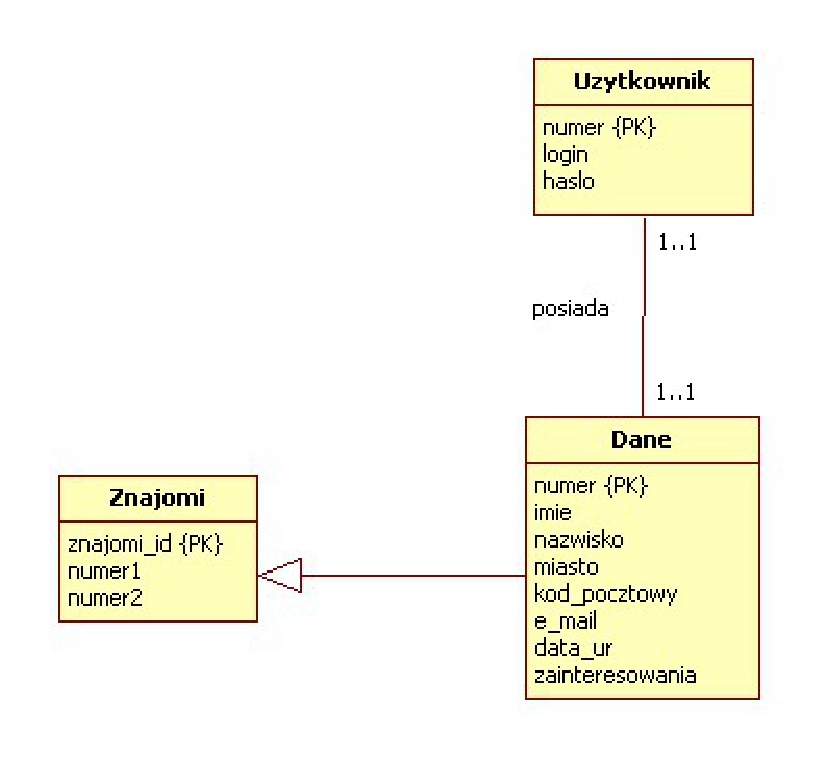
\includegraphics[scale=0.55]{Model.eps}
	      \end{center}
    \end{figure}
\end{center}

\section[Dokumentacja techniczna]{Dokumentacja techniczna}
\subsection[Serwer eTalk]{Serwer eTalk}
\subsubsection[Opis programu]{Opis programu}

\subsubsection[Opis klasy About]{Opis klasy About}
\texttt{About} jest publiczną klasą formularza dziedziczącą po klasie bibliotecznej \texttt{Form}
języka C\#. Formularz wyświetla informacje o programie i autorach.

\subsubsection[Opis klasy ClientRequest]{Opis klasy ClientRequest}
\texttt{ClientRequest} jest publiczną klasą odpowiedzialną za przetwarzanie żądań klienta, które są przesyłane w formacie XML.
Format wiadomości powinien być zgodny z protokołem komunikacji opisanym w tym dokumencie.\\
Metoda \texttt{getType} zwraca typ otrzymanej wiadomości.\\
Metoda \texttt{getParams} zwraca główne parametry otrzymanej wiadomości i ewentualnie dodatkowe parametry, jeżeli zostały przesłane. Parametry są przechowywane w obiekcie klasy \texttt{ClientRequestParams}.

\subsubsection[Opis klasy ClientRequestParams]{Opis klasy ClientRequestParams}
\texttt{ClientRequestParams} stanowi opakowanie dla głównych i ewentualnie dodatkowych parametrów żądania klienta w formacie XML. Zwracanie i ustawianie parametrów jest możliwe dzięki mechanizmowi indekserów (indeksowanie tablicy nazwami parametrów).

\subsubsection[Opis klasy GaduGadu]{Opis klasy GaduGadu}
\texttt{GaduGadu} jest publiczną klasą odpowiedzialną za obsługę protokołu komunikatora Gadu-Gadu.
Implementując klasę GaduGadu autorzy projektu wykorzystali możliwości darmowej biblioteki HAKGERSoft.
Metody \texttt{connect} i \texttt{disconnect} służą odpowiednio do łączenia się i rozłączania się z serwerem.
Operacja łącznia się z serwerem wiąże się z procesem uwierzytelniania klienta.\\
Metoda \texttt{sendMessage} pozwala na wysłanie pod dany numer, danej w parametrze procedury wiadomości.
Aby wysłać wiadomość użytkownik musi być uwierzytelniony.\\
Metoda \texttt{gadu\_GGMessageReceive} realizuje funkcję nasłuchiwacza przychodzących wiadomości do uwierzytelnionego użytkownika.\\
Metoda \texttt{changeStatus} zmienia status uwierzytelnionego użytkownika na status podany w pierwszym parametrze metody. Zmianie ulega również opis użytkownika. Nowy opis przekazywany jest jako drugi parametr metody.\\
Metoda \texttt{sendImage} wysyła obrazki wraz z wiadomością tekstową do adresata. W trakcie przesyłania obrazek jest pamiętany w strumieniu pamięci (obiekt bibliotecznej klasy \texttt{MemoryStream}). Klient powinien określić zawartość wiadomości tekstowej, numer adresata, pozycję obrazka w tekście, oraz sam obrazek przechowywany w obiekcie bibliotecznej klasy \texttt{Image} i przekazać te dane jako parametry metody.

\subsubsection[Opis klasy HandleClient]{Opis klasy HandleClient}
\texttt{HandleClient} jest publiczną klasą odpowiedzialną za obsługę żądań Klienta eTalk. Metoda \texttt{getMessage}
wykorzystując obiekt klasy bibliotecznej \texttt{NetworkStream} języka C\# pobiera żądanie klienta w formacie XML zgodne z opisanym w tym dokumencie poniżej protokołem komunikacji.\\
Wykorzystując obiekty klas \texttt{ClientRequest} i \texttt{ClientRequestParams} klasa przetwarza żądanie i jego parametry. \\
Po rozpoznaniu typu zapytania i jego parametrów klasa wykorzystując obiekt \texttt{QueryMaker} wykonuje zadaną operację w bazie danych. Po poprawnym wykonaniu zadania wysyła odpowiedź utworzoną przez obiekt klasy \texttt{MessageFactory}.\\
Klasa \texttt{HandleClient} przesyła odpowiedź klientowi wykorzystując obiekty bibliotecznych klas \texttt{StreamWriter} i \texttt{NetworkStream}.\\
Metoda \texttt{doChat} przesyła przekazaną w parametrze metody wiadomość do zadanego w parametrze metody użytkownika.

\subsubsection[Opis klasy ListenerWindow]{Opis klasy ListenerWindow}
\texttt{ListenerWindow} jest publiczną klasą formularza dziedziczącą po klasie bibliotecznej \texttt{Form}
języka C\#. Metoda wyświetla formularz zawierający dwa pole tekstowe przeznaczone na adres IP i numer portu.
Podane informacje jednoznacznie określają gniazdo nasłuchujące Serwera eTalk. Po potwierdzeniu wprowadzonych danych
program tworzy nowy obiekt klasy \texttt{Serwer} i rozpoczyna nasłuchiwanie na określonym porcie pod określonym adresem.

\subsubsection[Opis klasy LoginWindow]{Opis klasy LoginWindow}
\texttt{LoginWindow} jest publiczną klasą formularza dziedziczącą po klasie bibliotecznej \texttt{Form}
języka C\#. Metoda wyświetla formularz zawierający dwa pole tekstowe przeznaczone na nazwę użytkownika i hasło do bazy danych Serwera eTalk. Po potwierdzeniu danych następuje połączenie z bazą danych PostgreSQL.
Program tworzy nowy obiekt klasy bibliotecznej \texttt{NpgsqlConnection} i nawiązuje połączenie z bazą, której namiary podawane są w parametrze konstruktora.

\subsubsection[Opis klasy MainForm]{Opis klasy MainForm}
\texttt{MainForm} jest publiczną klasą głównego formularza aplikacji Serwer eTalk dziedziczącą po klasie bibliotecznej \texttt{Form} języka C\#. Klasa jest odpowiedzialna za wyświetlanie i konfigurowanie głównego
okna aplikacji, jego komponentów oraz obsługę wszystkich zdarzeń z nimi związanych.
Menu główne aplikacji jest obiektem klasy \texttt{MainMenu} i zawiera przyciski, które są obiektami
klasy \texttt{MenuItem}. Dolne menu jest obiektem klasy \texttt{StatusBar} i zawiera następujące komponenty -- obiekty
klasy \texttt{StatusBarPanel}:
\begin{itemize}
    \item[--] panel informacji o komponencie, na który użytkownik wskazuje kursorem myszy
(obsługa zdarzenia \texttt{Select});
    \item[--] panel z dniem tygodnia i datą (informacje pobrane z obiektu klasy \texttt{DateTime});
    \item[--] panel z godziną (informacje pobrane z obiektu klasy \texttt{Timer}, odświeżane co sekunda
dzięki obsłudze zdarzenia \texttt{Tick}).
\end{itemize}
Klasy \texttt{MainForm} użyto również do składowania głównych obiektów Serwera eTalk,
np. lista połączeń.\\
W centrum głównego formularza znajduje się lista (obiekt bibliotecznej klasy \texttt{ListBox}) wszystkich użytkowników z bazy danych aplikacji.
Poniżej opisanej listy znajduje się druga lista zawierająca rozszerzone informacje o użytkowniku wybranym z pierwszej listy (wykorzystano tutaj obsługę zdarzenia \texttt{SelectedIndexChanged} dla obiektu klasy \texttt{ListBox}). Obie listy można odświeżać.

\subsubsection[Opis klasy MessageFactory]{Opis klasy MessageFactory}
\texttt{MessageFactory} jest publiczną klasą służącą do wytwarzania odpowiedzi dla klienta.\\
Każda kolejna metoda klasy potrafi zwrócić odpowiedź o ustalonym typie i zadanych parametrach.\\
Wszystkie odpowiedzi są w formacie XML i są tworzone na podstawie protokołu komunikacyjnego, utworzonego specjalnie na potrzeby aplikacji eTalk. Dokładny opis protokołu znajduje się w dalszej części tego dokumentu.

\subsubsection[Opis klasy Pair]{Opis klasy Pair}
\texttt{Pair<T,U>} jest pomocniczą klasą generyczną przechowującą pary elementów.\\
Pierwszy element jest typu T, drugi element jest typu U.

\subsubsection[Opis klasy QueryMaker]{Opis klasy QueryMaker}
\texttt{QueryMaker} jest główną klasą wykonującą operacje na bazie danych PostgreSQL Serwera eTalk.\\
Do łączenia się bazą PostgreSQL autorzy projektu wykorzystali darmową bibliotekę \texttt{Npgsql} dla języka C\#.
Klasa \texttt{QueryMaker} posiada następujące metody:
\begin{itemize}
    \item[--] \texttt{addClient}, która dodaje nowego klienta do bazy. Informacje o nowym kliencie są zapisane w słowniku (obiekt klasy bibliotecznej \texttt{Dictionary<String,String>}). Metoda obsługuje każdą poprawną kombinację danych klienta (pewne pola mogą pozostać niewypełnione, reszta jest obowiązkowa).
              Metoda przetwarza relacje \texttt{uzytkownik} oraz \texttt{dane} i wykorzystuje polecenia \texttt{INSERT} i zapytania \texttt{SELECT} w języku SQL;
    \item[--] \texttt{changeStatus}, która zmienia stary status uwierzytelnionego klienta na nowy, zadany w drugim parametrze metody. Możliwe statusy to: \texttt{Dostepny}, \texttt{Niedostepny}, \texttt{Niewidoczny} i \texttt{Zaraz wracam}. Metoda przetwarza relację \texttt{uzytkownik} i wykorzystuje polecenie \texttt{UPDATE} w języku SQL;
    \item[--] \texttt{deleteClient}, która usuwa z bazy danych informacje o zadanym w parameterze kliencie.
              Metoda przetwarza relacje \texttt{uzytkownik} oraz \texttt{dane} i wykorzystuje polecenia \texttt{DELETE} w języku SQL;
    \item[--] \texttt{getClients}, która zwraca listę wszystkich użytkowników znalezionych w bazie Serwera eTalk.
              Metoda przeszukuje relację \texttt{uzytkownik} i wykorzystuje proste zapytanie \texttt{SELECT} w języku SQL;
    \item[--] \texttt{getClientDetail}, która zwraca dodatkowe dane klienta zadanego przez parametr metody.
              Metoda przeszukuje relację \texttt{dane} i wykorzytuje proste zapytanie \texttt{SELECT} w języku SQL;
    \item[--] \texttt{getFriends}, która zwraca listę znajomych klienta zadanego jako parametr metody. Lista zawiera pary postaci (numer\_klienta, pseudonim).
        Metoda przeszukuje relację \texttt{znajomi} i wykorzystuje proste zapytanie \texttt{SELECT} w języku SQL;
    \item[--] \texttt{login}, która sprawdza, czy podczas uwierzytelniania klient podał poprawną nazwę użytkownika i hasło. Metoda przeszukuje relację \texttt{uzytkownik} i wykorzystuje proste zapytanie \texttt{SELECT} w języku SQL;
    \item[--] \texttt{makeFriends}, która łączy dwóch nowych znajomych zadanych jako pierwsze dwa parametry metody oraz zapisuje drugiego klienta pod pseudonimem przekazanym do metody jako trzeci parametr. W efekcie drugi klient trafia na listę znajomych pierwszego klienta pod wybranym pseudonimem.  
        Metoda przetwarza relację \texttt{znajomi} i wykorzystuje polecenie \texttt{INSERT} i zapytanie \texttt{SELECT} w języku SQL;
    \item[--] \texttt{modifyClient}, która modyfikuje podstawowe i dodatkowe informacje o kliencie. Lista modyfikacji przekazywana jest w postaci słownika jako parametr metody.   
        Metoda przetwarza relacje \texttt{uzytkownik} oraz \texttt{dane} i wykorzystuje polecenia \texttt{UPDATE} i zapytania \texttt{SELECT} w języku SQL.
\end{itemize}

\subsubsection[Opis klasy Serwer]{Opis klasy Serwer}
\texttt{Serwer} jest publiczną klasą, która tworzy nowy obiekt klasy bibliotecznej \texttt{TcpListener} języka C\#, nasłuchuje w oczekiwaniu na klientów na gnieździe nasłuchującym i zwraca gniazdo połączone, gdy dojdzie do połączenia.
Klasa \texttt{Serwer} tworzy nowy obiekt klasy \texttt{HandleClient} przekazując jej w parametrze konstruktora gniazdo połączone -- obiekt bibliotecznej klasy \texttt{Socket} języka C\# oraz numer porządkowy klienta (liczy się kolejność połączeń). Serwer jest aplikacja wielowątkową. Proces macierzysty tworzy wątki do obsługi każdego klienta z osobna. Dzięki zrównoleglonej obsłudze poszczególnych klientów, Serwer eTalk działa szybciej.


\subsection[Klient eTalk]{Klient eTalk}
\subsubsection[Opis programu]{Opis programu}

\subsubsection[Opis klasy About]{Opis klasy About}
\texttt{About} jest publiczną klasą formularza dziedziczącą po klasie bibliotecznej \texttt{Form}
języka C\#. Formularz wyświetla informacje o programie i autorach.

\subsubsection[Opis klasy MessageFactory]{Opis klasy MessageFactory}
\texttt{MessageFactory} jest publiczną klasą służącą do wytwarzania żądań dla klienta.\\
Każda kolejna metoda klasy potrafi zwrócić żądanie o ustalonym typie i zadanych parametrach.\\
Wszystkie żądania są w formacie XML i są tworzone na podstawie protokołu komunikacyjnego, utworzonego specjalnie na potrzeby aplikacji eTalk. Dokładny opis protokołu znajduje się w dalszej części tego dokumentu.

\subsubsection[Opis klasy ServerResponse]{Opis klasy ServerResponse}
\texttt{SerwerResponse} jest publiczną klasą odpowiedzialną za przetwarzanie odpowiedzi serwera, które są przesyłane w formacie XML.
Format wiadomości powinien być zgodny z protokołem komunikacji opisanym w tym dokumencie.\\
Metoda \texttt{getType} zwraca typ otrzymanej wiadomości.\\
Metoda \texttt{getParams} zwraca główne parametry otrzymanej wiadomości i ewentualnie dodatkowe parametry, jeżeli zostały przesłane. Parametry są przechowywane w obiekcie klasy \texttt{SerwerResponseParams}.

\subsubsection[Opis klasy ServerResponseParams]{Opis klasy ServerResponseParams}
\texttt{SerwerResponseParams} stanowi opakowanie dla głównych i ewentualnie dodatkowych parametrów odpowiedzi klienta w formacie XML. Zwracanie i ustawianie parametrów jest możliwe dzięki mechanizmowi indekserów (indeksowanie tablicy nazwami parametrów).

\subsection[Opis protokołu komunikacyjnego aplikacji eTalk]{Opis protokołu komunikacyjnego aplikacji eTalk}

\section[Raport z przeprowadzonych testów]{Raport z przeprowadzonych testów}
\subsection[Test 1.]{Test 1.}


\section[Przyszły rozwój aplikacji]{Przyszły rozwój aplikacji}
\subsection[Obsługa protokołu Gadu-Gadu]{Obsługa protokołu Gadu-Gadu}


\begin{thebibliography}{9}
\bibitem{OU} http://www.seoteka.pl/a85.php (ostatni dostęp do strony 2010-04-12)
\bibitem{PO} \emph{Polityka}, nr. 11 (2747), 2010-03-13
\bibitem{ST} S.Turkle, \emph{Life on the Screen}, Simon \& Schuster, 1997
\bibitem{GG} http://info.gadu-gadu.pl/producent/historia (ostatni dostęp do strony 2010-04-12)
\bibitem{ID} http://www.pcworld.pl/artykuly/41638/Lepsze.niz.Gadu.Gadu.html (ostatni dostęp do strony 2010-04-12)
\bibitem{TL} http://firma.o2.pl/ (ostatni dostęp do strony 2010-04-12)
\end{thebibliography}
\end{document} 